\documentclass[tikz,convert]{standalone}
\usepackage{tikz}
\usetikzlibrary{backgrounds}
\usetikzlibrary{arrows}
\usetikzlibrary{automata}

\usetikzlibrary{snakes}
\tikzset{
  treenode/.style = {align=center, inner sep=0pt, text centered,
    font=\sffamily},
  idle/.style = {treenode, circle, black, font=\sffamily\bfseries, draw=black,
  	text width=1.5em},
  sel_n/.style = {treenode, circle, white, font=\sffamily\bfseries, draw=black,
    fill=black, text width=1.5em},% arbre rouge noir, noeud noir
  opponent_n/.style = {treenode, circle, fill=black, text=white,
     text width=1em, very thick},% arbre rouge noir, nil
  prob_n/.style = {treenode, circle, fill=black,
     text width=1em, very thick},% arbre rouge noir, nil
   prob_reg_n/.style = {treenode, circle, red, draw=red, fill=black,
 	text width=1em, very thick},% arbre rouge noir, nil
    prob_gen_n/.style = {treenode, circle, blue, draw=blue, fill=blue,
 	text width=1em, very thick},% arbre rouge noir, nil
  reg_n/.style = {treenode, circle, red, draw=red, 
    text width=1.5em, very thick},% arbre rouge noir, noeud rouge
  gen_n/.style = {treenode, circle, draw=blue,
    text width=1.5em, very thick},% arbre rouge noir, nil
  sim_n/.style = {treenode, circle, draw=pink,
	text width=1.5em, very thick},% arbre rouge noir, nil
  updated_n/.style = {treenode, circle, draw=green,
  	text width=1.5em, very thick},% arbre rouge noir, nil
  example_n/.style = {treenode, circle, draw=green,
  	text width=2.5em, font=\small, very thick},% arbre rouge noir, nil
}

\newcommand{\prob}[3]{\small $P_{#1}(#2|#3)$}


\begin{document}
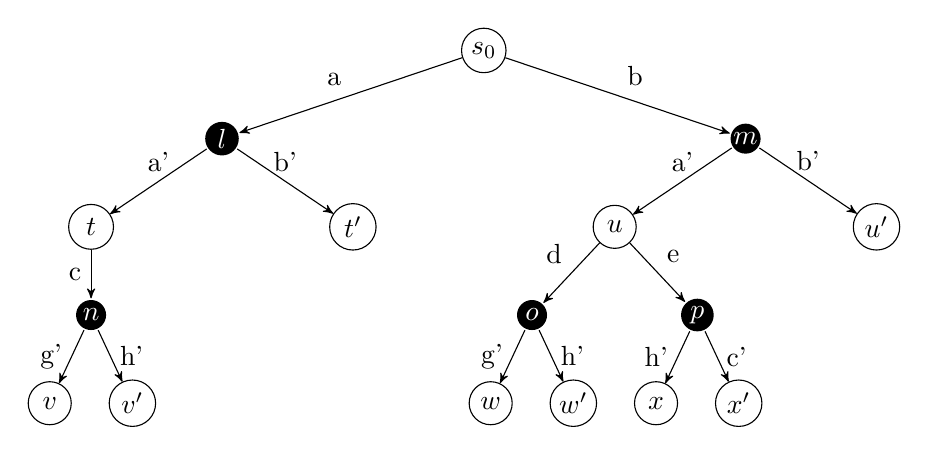
\begin{tikzpicture}[->,>=stealth',level/.style={sibling distance = 9.5cm/#1,
	level distance = 1.6cm},scale=0.7] 

%\tikzstyle{level 1}=[sibling distance=9cm]
%\tikzstyle{level 2}=[sibling distance=4cm]
\tikzstyle{level 3}=[sibling distance=3cm]
\tikzstyle{level 4}=[sibling distance=1.5cm]
\tikzstyle{level 5}=[sibling distance=1cm]
\node [idle] {$s_0$}
child{ node [opponent_n] {$l$} 
	child{ node [idle] {$t$} 
		child{ node [opponent_n] {$n$}	
				child{ node [idle] {$v$} 
				edge from parent node[left] {g'}
			} 
			child{ node [idle] {$v'$}         
				edge from parent node[right] {h'}    
			}
			edge from parent node[left] {c}
		}
		edge from parent node[anchor=south] {a'}
	}
	child{ node [idle] {$t'$}
		edge from parent node[anchor=south] {b'}
	}                            
	edge from parent node[above left] {a} 
}   
child{ node [opponent_n] {$m$}
	child{ node [idle] {$u$} 
		child{ node [opponent_n] {$o$}
			child{ node [idle] {$w$}
				edge from parent node[left] {g'}
			}
			child{ node [idle] {$w'$}
				edge from parent node[right] {h'}
			}
			edge from parent node[above left] {d}
		}
		child{ node [opponent_n] {$p$} 
			child{ node [idle] {$x$}
				edge from parent node[left] {h'}
			}
			child{ node [idle] {$x'$}
				edge from parent node[right] {c'}
			}
			edge from parent node[above right] {e}
		}
		edge from parent node[anchor=south] {a'}
	} 
	child{ node [idle] {$u'$}         
		edge from parent node[anchor=south] {b'}    
	}
	edge from parent node[above right] {b}
}

; 
\end{tikzpicture}
\end{document}